% !TEX root = C:\Users\Jan\Documents\dev\Risk-Measurement-Framework\masterthesis_tex\masterthesis_main.tex
\section{Implementation}
\label{sec:implementation}

Afer explaining and discussing the concept of the RMF in section \ref{sec:conFrame}, this section describes the implementation of the technical framework RMF by following the procedures of ISO 27004 \cite{ISO_27004_2009}. The technical RMF uses Python 3.7 \cite{10.5555/1593511} as the programming language and ART to implement the attacks. As already mentioned in subsection \ref{sec:approaches} this technical RMF should be used a step ahead of using the framework of Schwerdtner et al. \cite{DBLP:journals/corr/abs-2011-04328}.

\subsection{Structure of the RMF}

\subsubsection*{Directory tree}

The RMF is structured as follows: \\

\dirtree{%
.1 rmf/.
.2 attacks/.
.3 art/.
.4 backdoors.py.
.2 backdoors/.
.3 png-Files.
.2 measurement/.
.3 monitoring.py.
.3 log.py.
.3 measurement.py.
.2 visualizations/.
.3 plot.py.
.2 log\_file.log.
.2 case\_study.py.
}

\hfill \break \noindent The \textit{png-Files} are used by the \textit{backdoors.py} script to add the backdoor patterns into the images which are the backdoor triggers. Both folders \textit{measurement} and \textit{metrics} contain implementations to monitor the collected data for the risk measurement and evaluate it. The \textit{plot.py} script generates the risk matrices and has a function to visualize the training dataset.

\subsection{Backdoor attacks from the ART}
\label{sec:impl_backdoor_attacks}

The following three attacks are all based on the ART \cite{art2018} and represent white-box and black-box attacks and both targeted and untargeted attacks. These attacks are the main factor to assign the values to the base measures. The attacks already differentiate between the original and poisoned dataset for evaluation.
All backdoor attacks use the \textit{Pattern Backdoor Attack} \cite{DBLP:journals/corr/abs-1708-06733} class which expects a pattern argument. The pattern is a picture which is for the poisoned images in the training dataset. The pattern must be implemented before training and choose a random selection of images. This is implemented in the RMF as follows:

\begin{lstlisting}
  n_train = np.shape(x)[0]
  num_selection = num_of_rand_images
  random_selection = np.random.choice(n_train, num_selection)
  x = x[random_selection]
  y = y[random_selection]
\end{lstlisting}

Then the arguments $x$ and $y$ are passed to the poisoning function from the ART. $x$ and $y$ are parameters which the function expects when calling it. Appendix \ref{sec:frame_func}
describe the functions and parameters. Further it is important that the shape of the images from the training dataset are \textit{N, H, W, C} or \textit{N, C, H, W}. $N$ is the number of
images in the batch, $H$ is the image height, $W$ is the image width, and $C$ is the channel number of an image such as grayscale or RGB. After adding a backdoor as a pattern to the
random images, the poisoned images are replaced back to the training dataset. These poisoned images are saved in a different folder to check if the images are missclassified after or while
testing the ML model.\\

The first attack uses the \textit{Pattern Backdoor Attack} class without any other backdoor classes from the ART. This attack which bases on Gu et al. \cite{DBLP:journals/corr/abs-1708-06733} is a black-box attack which is untargeted. In the RMF the attack is implemented with a pattern backdoor only which Figure \ref{fig:original_example} and Figure \ref{fig:poisoned_example} show as the
difference between the original and the poisoned image. The goal of this attack is to change the original label to a random other label. This attack can be executed without any
information because it is not important which training dataset the ML model use and what ML model is used for the training itself. \\

After poisoning the images these image need be copied back into the original training dataset. Before this can be done, the poisoned data must replace the original training dataset which contains
no backdoors. After taking the RMF the random original images, the RMF saves them into a temporary variable and then delete the images from the original training dataset. The next step is the
poisoning while the poisoned data and the original training dataset need the same shape and dimension which make it possible to copy the poisoned images. As mentioned before the poisoning
function takes four specific shapes which make it easy to have the same shape in the original training dataset and poisoned data. The implementation of the attack additionally shows the
effort an attacker have to implement this attack. Thus the steps can be used for the attacker's knowledge.

\begin{figure}[!ht]
  \centering
  \begin{minipage}[b]{0.4\textwidth}
    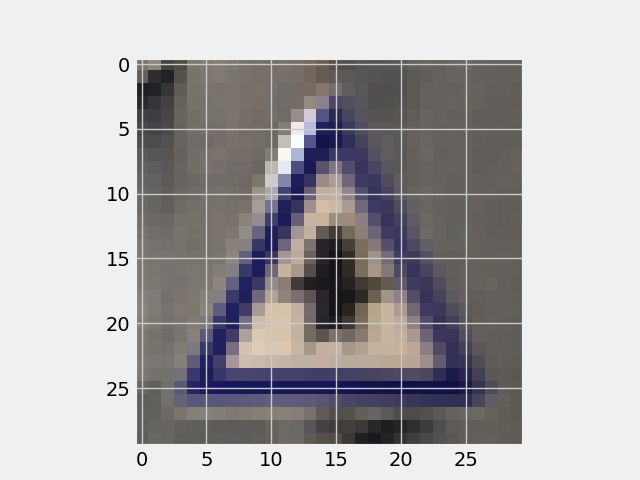
\includegraphics[width=8cm]{pictures/original_example.png}
    \caption{Street sign without a backdoor pattern with the label \textit{Right-of-way at intersection}.}
    \label{fig:original_example}
  \end{minipage}
  \hfill
  \begin{minipage}[b]{0.4\textwidth}
    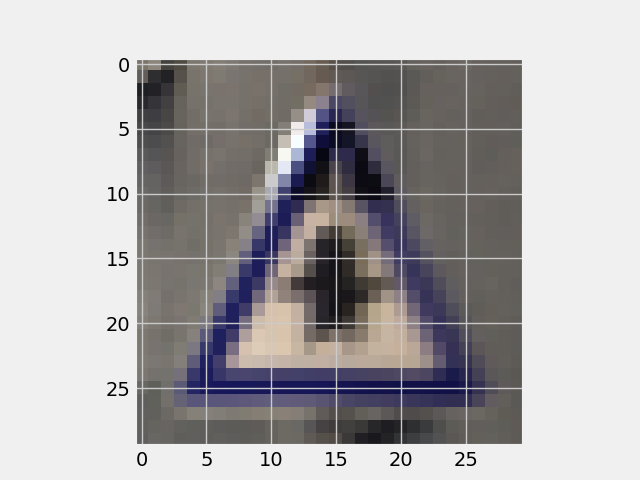
\includegraphics[width=8cm]{pictures/poisoned_example.png}
    \caption{Street sign with a backdoor pattern but still with the original label \textit{Right-of-way at intersection}.}
    \label{fig:poisoned_example}
  \end{minipage}
\end{figure}

The problem with this attack is that the ART can load the backdoor into the selected images, but the poisoned images are not mixed into the original training dataset. \\
The \textit{Clean Label Backdoor Attack} \cite{turner2018clean} poison images and missclassify during the training time. To use this attack the \textit{Pattern Backdoor Attack} must be
used before and then the clean label attack can be executed after training. After adding the backdoor trigger with \textit{Pattern Backdoor Attack} the original training dataset are trained
with a proxy classifier which should do the same classification tasks as the original classifier.

The \textit{Hidden Trigger Backdoor Attack} \cite{DBLP:journals/corr/abs-1910-00033} need to be executed after training. To add the backdoor, the \textit{Pattern Backdoor Attack} must be
used before. After training, the poisoned data and a smaller number of clean training inputs are used to finetune the model. Finetuning means, adjusting parameters of the ML model to
improve it with a small amount of training dataset to improve the performance \cite{DBLP:conf/acl/LiWTTTPBCA20}, \cite{DBLP:journals/corr/abs-2112-08691}. For the attack the poisoned data
are used with a small amount of clean training dataset. The following Python code shows the finetuning of a ML model where the attack is implemented.

\begin{lstlisting}
  dataset_size = size
  num_labels = label_size
  num_per_label = dataset_size/num_labels

  poison_dataset_inds = []

  for i in range(num_labels):
      label_inds = np.where(np.argmax(y_train, axis=1) == i)[0]
      num_select = int(num_per_label)
      if np.argmax(target) == i:
          num_select = int(num_select - min(num_per_label, len(poison_data)))
          poison_dataset_inds.append(poison_indices)

      if num_select != 0:
          poison_dataset_inds.append(np.random.choice(label_inds, num_select, replace=False))

  poison_dataset_inds = np.concatenate(poison_dataset_inds)

  poison_x = np.copy(x_train)
  poison_x[poison_indices] = poison_data
  poison_x = poison_x[poison_dataset_inds]

  poison_y = np.copy(y_train)[poison_dataset_inds]
\end{lstlisting}

The parameters of the \textit{Hidden Trigger Backdoor Attack} are analog to the \textit{Clean Label Backdoor Attack} but the pattern is different as the backdoor trigger which Figure \ref{fig:poisoned_hidden_trigger} shows.

\begin{figure}[ht!]
  \centering
  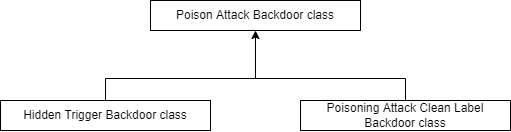
\includegraphics[width=9cm]{pictures/attack_relationship.png}
  \caption{Both attack classes (\textit{Clean Label Backdoor Attack} and \textit{Hidden Trigger Backdoor Attack}) get the backdoor from the \textit{Pattern Backdoor Attack}.}
  \label{fig:attack_relationship}
\end{figure}

\subsection{Measurement methods to assign values to the risk indicators}

The risk indicators are the main part for the risk measurement. Every risk indicator is implemented as an own function in the RMF in a class that represents the object. These functions make it possible to measure the risk indicator values at each step during the ML model training. The object classes represent the measurement methods to separate the risk indicator functions. \\
The $accuracy=\frac{n(correctly\_predicted)}{n(all)}$ is implemented as Nguyen and Zeigermann \cite{9783960101925} describe it. The next implemented risk indicator is the attack time, which measures the time an attack needs to be executed and how long it takes to train the ML model with the poisoned training dataset. The attack time also measure if the attack is executed during training or inference time. \\
Attack specificity is a risk indicator that measures if the attack is targeted or untargeted. The ART attacks have a parameter that takes a target. If the target is random, then there is no specific label. If the attack is targeted, there is a specific label with a certain number of images in percentage which poison images. The TP, TN, FP, FN risk indicator can be measured by getting these values from the confusion matrix. Keras show these values with a implemented function from Scikit-learn \cite{scikit-learn} in the RMF. The computational resources get the values from the operating system for the specific executed Python script. The attacker's knowledge will be implemented based on the executed attack. For example, if the \textit{Pattern Backdoor Attack} is executed in the ML model, then the function for the attacker's knowledge returns the steps to implement this specific attack \cite{bsi_2013}. Attacker's goal \cite{DBLP:journals/corr/abs-2012-04884} can return the steps to do an inference failure, obtain secret information, or executing a denial-of-service. An inference failure happens during the testing phase. If an attacker tries to execute an inference failure he could use exploratory attacks \cite{tabassi2019taxonomy} or evasion attacks \cite{DBLP:conf/sp/Carlini017}. Obtain secret information can be, for example, stealing model attacks \cite{DBLP:journals/corr/abs-2105-00623}, \cite{DBLP:journals/wicomm/ZhangLGQTZ20}. Denial-of-service attacks have the goal to slow down the ML model or crash the ML model completly \cite{DBLP:journals/sensors/VaccariAC20}. If one of these goals is identified, then the attacker's goal function returns pre-determined steps on how to achieve this goal. If an attacker tries to missclassify the ML model based on backdoor attacks, then the goal is an inference failure because the image classification fails during inference time. To achieve this goal the attacker has to develop a backdoor attack. The difference between achieving this goal and getting the knowledge of the attacker is about how they develop the backdoor attack to achieve the goal and how much the attacker knows to implement the attack into the ML model. The attacker's goal do not concentrate on specific attacks, only on what the attacker has to do generally. \\
Subsection \ref{sec:impl_backdoor_attacks} explains how the attacks in the measurement methods will be implemented.

\subsection{Implementing the measurement construct}

After assigning the risk indicators based on the threat model of Doynikova et al. \cite{DBLP:conf/crisis/DoynikovaNGK20}, this subsection explains the implemented measurement construct starting from the base measures up to the decision criteria. \\
The measurement function is a single function which takes the base measures that has to be combined to the derived measures. To access these base measures, they must first be separated from the base measures that are given directly to the analytical model function. Figure \ref{fig:impl_meas_func} visualizes the procedure of the measurement function. The first measurement function calculates the derived measures of the TP, TN, FP, FN into the ML metrics such as F1-Score, precision-recall, and confusion matrix with the mathematical functions from Nguyen and Zeigermann \cite{9783960101925}. These ML metrics show the total results of the ML model's performance and represent how the attacked changed their values as total results.
Since the value of the $Risk$ should represent a higher risk at a high value than at a low value, the base measures as well as derived measures must yield corresponding results. In order to ensure this representation, it is important for the accuracy, F1-Score, precision-recall, and confusion matrix that their reduced values due to the attack are used as high values for the risk. Since the accuracy and the other ML metrics are represented as percentages and thus lie between $0$ and $100\%$ or $0$ and $1$, the RMF reverses these values. If the accuracy
is for example $0.06$ or $6\%$, the RMF converts this value to $0.94$ out of $1$. This allows the value to appropriately reflect how much the accuracy increases the overall $Risk$. To calculate the derived measure for the extent of damage the last value calculates how much labels are missclassified. This matching is implemented by key-value pairs whereby the key is the original predicted image and the value is the poisoned predicted image. If the poisoned prediction is the correct missclassified target label, then a counter increases. Then the result of this matching can be compared with the possible number of poisoned images to check how much images are actually poisoned. The resulting percentage reflects how effective the attack was on the tested ML model. \\
In order not to depend on the different ML libraries, the RMF gets its own functions of the different ML metrics. The next function in Figure \ref{fig:impl_meas_func} add all attack steps together.

\begin{figure}[ht!]
  \centering
  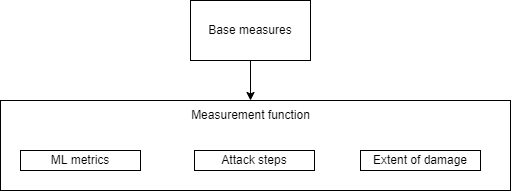
\includegraphics[width=10cm]{pictures/impl_meas_func.png}
  \caption{The measurement function takes the base measures and distributes them to the inner measurement functions.}
  \label{fig:impl_meas_func}
\end{figure}

\subsubsection*{Mapping between the base measures}

The attack time and specificity are the only risk indicators which have to be mapped to the attacker's knowledge and goal. Based on the low-level attributes, the high-level attributes are additionally adjusted after the measurement. After the execution of the attacks, the values of the attack itself - specifically the attack time - is used to measure the time an attacker need to execute its attack \cite{DBLP:journals/corr/abs-2012-04884}. This measurement is based on the difference between training of the ML model without and with the attack. The attack time for measuring the extent of damage is used to see which vulnerabilities a ML model has during the training or inference time \cite{DBLP:journals/csur/RosenbergSER21}. Since the values that are measured can be used to measure the effort of an attacker, this risk indicator must be mapped. \\
For the attack specificity, the RMF measures how much images are poisoned and what the attacker has to do to poison targeted images \cite{DBLP:conf/iccv/ZhuNXWW21} or how he poisons random images \cite{DBLP:journals/corr/abs-1708-06733}. The attack specificity measures the steps to poison images to a target goal based on the target label that the ART takes as an argument for the attack. These steps are mapped with the attacker's knowledge and goal to calculate all steps that the attacker has to perform.
The following subsection describes how the results from the measurement methods are evaluated in the measurement construct.

\subsubsection*{The analytical models}

Figure \ref{fig:impl_ana_mod} shows the procedure of the analytical model. The analytical model takes the base measures that are not calculated into derived measures and the derived measures from the measurement function. All values for the risk calculation are combined here and calculated to get the probability of occurrence and the extent of damage. \\ It is important to note that the measurement of the effectiveness of the attack is obtained using the predictions from the test dataset, since during the attack at training time both the original and the poisoned training datasets may not differ from the labels.

\begin{figure}[ht!]
  \centering
  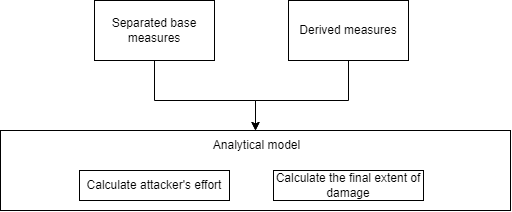
\includegraphics[width=10cm]{pictures/impl_ana_mod.png}
  \caption{The analytical model takes the separated base measures and derived measures. Then it distributes them to the inner analytical models.}
  \label{fig:impl_ana_mod}
\end{figure}

\subsubsection*{The decision criteria}

The last step to get the measurement results is shown in Figure \ref{fig:impl_dec_criteria} which input for the decision criteria are the two output values from Figure \ref{fig:impl_ana_mod}. The attacker's effort has to be in an interval which has to be specified as an information need. The extent of damage must also be checked based on an information need \cite{ISO_27004_2009}. For this thesis there is no interval because the information need is not considered further. If the criteria is fulfilled the indicators are able to be calculated and then the result can be depicted. This procedure is described in subsection \ref{sec:impl_meas_res}.

\begin{figure}[ht!]
  \centering
  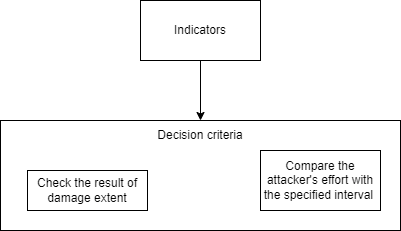
\includegraphics[width=10cm]{pictures/impl_dec_criteria.png}
  \caption{The analytical model takes the separated base measures and derived measures. Then it distribute them to the inner analytical models.}
  \label{fig:impl_dec_criteria}
\end{figure}

\subsection{Visualizing the measurement results with the RMF}
\label{sec:impl_meas_res}

\subsubsection*{The logging function}

To show all steps of the risk measurement, the RMF has a function that documents them. Assigned values of the risk indicators, the pre-determined steps to measure the attacker's effort, and the calculations of the risk measurement are represented with an optimized logging function, based on the Python logging module. The function takes two arguments such as a message string and the wanted logging level (i.e. INFO or DEBUG). The following example shows an execution of the logging function:

\begin{lstlisting}
  log(f"{variable_name}", 'INFO')
\end{lstlisting}

This function should make it possible for human judgment to find the critical parts where the ML model is particularly vulnerable for backdoor attacks. The next section evaluates the implemented concept from this section and present the results of a case study which uses the RMF to measure risks of a ML model backdoor attack.

\subsubsection*{Plotting the risk matrix}

The measurement results show the monitored data based on the measurement process of ISO 27004 \cite{ISO_27004_2009}. This contains all logged risk indicator values and visualized ML metrics. A second part will show the risk for the ML model with an attack. The risk will be calculated by $Risk = $ \textit{Extent of damage} $*$ \textit{Probability of occurence} \cite{DBLP:journals/access/JianxingHSH21}. This risk value must be depicted in a risk matrix which shows how high the risk is with the executed attack. Based on the measurement result it should be possible to interpret the attack, but the RMF shows no defense methods. The RMF concentrates only on the attack and the associated risk measurement. What happens with these results and what they are used for remains open. The following section evaluates the RMF risk measurement based on a case study. This case study trains a ML model for street sign classification on autonomous driving which is attacked by a backdoor attack.
